 \documentclass[12pt]{article}
% import preamble
% My custom preamble. 
% Import this into main.tex doc with % My custom preamble. 
% Import this into main.tex doc with % My custom preamble. 
% Import this into main.tex doc with \input{preamble} after class definition
\usepackage[utf8]{inputenc}
% MATH
\usepackage{amsmath}
\usepackage{amssymb}
\usepackage{graphicx}
\usepackage{mathrsfs}
\usepackage{commath}
% [physics] contains nice derivative commands
\usepackage{physics}
% [bbold] contains doublestroke characters but overwrites several commands like \mathbb
% \usepackage{bbold}
% [cancel] allows the \cancelto{0}{x} command
\usepackage{cancel}
% adjusts height of the '\\' command for line breaks
\setlength{\jot}{10pt}


% FORMATTING
% this adjusts margins
% new margins for all pages
%\usepackage[bottom=.6in,top=.6in]{geometry}
% \newgeometry and \restoregeometry for page specific margins
\usepackage{geometry}
\usepackage[titletoc]{appendix}
\usepackage{caption}
\usepackage{float}
\usepackage{titling}
% [lscape] for making landscape pages \begin{landscape}
\usepackage{lscape}
% for subfigures (better than minipages)
% EX: \begin{subfigure}[t]{0.45\textwidth}
\usepackage{subcaption}
% for fancy tables
\usepackage{ragged2e}
\usepackage{array}
% define new column types for tabular environments
% these wrap text but you have to specify column width
% ex: \begin{tabular}{|L{4cm}|L{2cm}}
\newcolumntype{L}[1]{>{\raggedright\let\newline\\\arraybackslash\hspace{0pt}}m{#1}}
\newcolumntype{C}[1]{>{\centering\let\newline\\\arraybackslash\hspace{0pt}}m{#1}}
\newcolumntype{R}[1]{>{\raggedleft\let\newline\\\arraybackslash\hspace{0pt}}m{#1}}

% making hyperlinks throughout the document
\usepackage[linktocpage=true, breaklinks=true]{hyperref}
\hypersetup{
    colorlinks,
    citecolor=blue,
    filecolor=blue,
    linkcolor=blue,
    urlcolor=blue
}
\usepackage{lmodern}  % for bold teletype font
\usepackage{xcolor}   % for \textcolor
% lstlisting environment settings
\usepackage{listings}
\lstset{
  basicstyle=\ttfamily,
  columns=fullflexible,
  frame=single,
  breaklines=true,
  postbreak=\mbox{\textcolor{red}{$\hookrightarrow$}\space},
  showstringspaces=false,
  keepspaces=true,
  commentstyle=\color{gray},
  keywordstyle=\color{blue},
  stringstyle=\color{green},
  numbers=left
}

% changing name of abstract here
\renewcommand{\abstractname}{Yung Salad}

% SQUARE ROOT TAIL CODE

\usepackage{letltxmacro}
\makeatletter
\let\oldr@@t\r@@t
\def\r@@t#1#2{%
\setbox0=\hbox{$\oldr@@t#1{#2\,}$}\dimen0=\ht0
\advance\dimen0-0.4\ht0
\setbox2=\hbox{\vrule height\ht0 depth -\dimen0}%
{\box0\lower0.4pt\box2}}
\LetLtxMacro{\oldsqrt}{\sqrt}
\renewcommand*{\sqrt}[2][\ ]{\oldsqrt[#1]{#2}}
\makeatother


 after class definition
\usepackage[utf8]{inputenc}
% MATH
\usepackage{amsmath}
\usepackage{amssymb}
\usepackage{graphicx}
\usepackage{mathrsfs}
\usepackage{commath}
% [physics] contains nice derivative commands
\usepackage{physics}
% [bbold] contains doublestroke characters but overwrites several commands like \mathbb
% \usepackage{bbold}
% [cancel] allows the \cancelto{0}{x} command
\usepackage{cancel}
% adjusts height of the '\\' command for line breaks
\setlength{\jot}{10pt}


% FORMATTING
% this adjusts margins
% new margins for all pages
%\usepackage[bottom=.6in,top=.6in]{geometry}
% \newgeometry and \restoregeometry for page specific margins
\usepackage{geometry}
\usepackage[titletoc]{appendix}
\usepackage{caption}
\usepackage{float}
\usepackage{titling}
% [lscape] for making landscape pages \begin{landscape}
\usepackage{lscape}
% for subfigures (better than minipages)
% EX: \begin{subfigure}[t]{0.45\textwidth}
\usepackage{subcaption}
% for fancy tables
\usepackage{ragged2e}
\usepackage{array}
% define new column types for tabular environments
% these wrap text but you have to specify column width
% ex: \begin{tabular}{|L{4cm}|L{2cm}}
\newcolumntype{L}[1]{>{\raggedright\let\newline\\\arraybackslash\hspace{0pt}}m{#1}}
\newcolumntype{C}[1]{>{\centering\let\newline\\\arraybackslash\hspace{0pt}}m{#1}}
\newcolumntype{R}[1]{>{\raggedleft\let\newline\\\arraybackslash\hspace{0pt}}m{#1}}

% making hyperlinks throughout the document
\usepackage[linktocpage=true, breaklinks=true]{hyperref}
\hypersetup{
    colorlinks,
    citecolor=blue,
    filecolor=blue,
    linkcolor=blue,
    urlcolor=blue
}
\usepackage{lmodern}  % for bold teletype font
\usepackage{xcolor}   % for \textcolor
% lstlisting environment settings
\usepackage{listings}
\lstset{
  basicstyle=\ttfamily,
  columns=fullflexible,
  frame=single,
  breaklines=true,
  postbreak=\mbox{\textcolor{red}{$\hookrightarrow$}\space},
  showstringspaces=false,
  keepspaces=true,
  commentstyle=\color{gray},
  keywordstyle=\color{blue},
  stringstyle=\color{green},
  numbers=left
}

% changing name of abstract here
\renewcommand{\abstractname}{Yung Salad}

% SQUARE ROOT TAIL CODE

\usepackage{letltxmacro}
\makeatletter
\let\oldr@@t\r@@t
\def\r@@t#1#2{%
\setbox0=\hbox{$\oldr@@t#1{#2\,}$}\dimen0=\ht0
\advance\dimen0-0.4\ht0
\setbox2=\hbox{\vrule height\ht0 depth -\dimen0}%
{\box0\lower0.4pt\box2}}
\LetLtxMacro{\oldsqrt}{\sqrt}
\renewcommand*{\sqrt}[2][\ ]{\oldsqrt[#1]{#2}}
\makeatother


 after class definition
\usepackage[utf8]{inputenc}
% MATH
\usepackage{amsmath}
\usepackage{amssymb}
\usepackage{graphicx}
\usepackage{mathrsfs}
\usepackage{commath}
% [physics] contains nice derivative commands
\usepackage{physics}
% [bbold] contains doublestroke characters but overwrites several commands like \mathbb
% \usepackage{bbold}
% [cancel] allows the \cancelto{0}{x} command
\usepackage{cancel}
% adjusts height of the '\\' command for line breaks
\setlength{\jot}{10pt}


% FORMATTING
% this adjusts margins
% new margins for all pages
%\usepackage[bottom=.6in,top=.6in]{geometry}
% \newgeometry and \restoregeometry for page specific margins
\usepackage{geometry}
\usepackage[titletoc]{appendix}
\usepackage{caption}
\usepackage{float}
\usepackage{titling}
% [lscape] for making landscape pages \begin{landscape}
\usepackage{lscape}
% for subfigures (better than minipages)
% EX: \begin{subfigure}[t]{0.45\textwidth}
\usepackage{subcaption}
% for fancy tables
\usepackage{ragged2e}
\usepackage{array}
% define new column types for tabular environments
% these wrap text but you have to specify column width
% ex: \begin{tabular}{|L{4cm}|L{2cm}}
\newcolumntype{L}[1]{>{\raggedright\let\newline\\\arraybackslash\hspace{0pt}}m{#1}}
\newcolumntype{C}[1]{>{\centering\let\newline\\\arraybackslash\hspace{0pt}}m{#1}}
\newcolumntype{R}[1]{>{\raggedleft\let\newline\\\arraybackslash\hspace{0pt}}m{#1}}

% making hyperlinks throughout the document
\usepackage[linktocpage=true, breaklinks=true]{hyperref}
\hypersetup{
    colorlinks,
    citecolor=blue,
    filecolor=blue,
    linkcolor=blue,
    urlcolor=blue
}
\usepackage{lmodern}  % for bold teletype font
\usepackage{xcolor}   % for \textcolor
% lstlisting environment settings
\usepackage{listings}
\lstset{
  basicstyle=\ttfamily,
  columns=fullflexible,
  frame=single,
  breaklines=true,
  postbreak=\mbox{\textcolor{red}{$\hookrightarrow$}\space},
  showstringspaces=false,
  keepspaces=true,
  commentstyle=\color{gray},
  keywordstyle=\color{blue},
  stringstyle=\color{green},
  numbers=left
}

% changing name of abstract here
\renewcommand{\abstractname}{Yung Salad}

% SQUARE ROOT TAIL CODE

\usepackage{letltxmacro}
\makeatletter
\let\oldr@@t\r@@t
\def\r@@t#1#2{%
\setbox0=\hbox{$\oldr@@t#1{#2\,}$}\dimen0=\ht0
\advance\dimen0-0.4\ht0
\setbox2=\hbox{\vrule height\ht0 depth -\dimen0}%
{\box0\lower0.4pt\box2}}
\LetLtxMacro{\oldsqrt}{\sqrt}
\renewcommand*{\sqrt}[2][\ ]{\oldsqrt[#1]{#2}}
\makeatother




\title{MoonRanger 4-Wheeled Kinematics Model}
\author{Ben Kolligs}
\date{\today}

\begin{document}

\maketitle

\section{Introduction}
In order to estimate MoonRanger's pose and generate motion from drive arcs we can use a kinematic model. 
The  model takes wheel velocities and determines the rover's body frame velocity, and vice versa. 
This document outlines a kinematic model for MoonRanger that is 4-wheeled, 3D, and offers a method for estimation of slip based off of terrain parameters. 
The main reference for the method presented here is the work of Neal Seegmiller in his PhD thesis, \cite{Seegmiller-2014-7945}. 
Note that throughout this document, we use the terms actuation kinematics to describe solving for joint rates given body velocity, and navigation kinematics to describe solving for body velocity given joint rates. 

\section{Development of Method}
\subsection{Transformation based kinematics}
The first step of formulating the kinematics is to define a transform table defining the actuated joints of MoonRanger. 
\begin{table}[H]
    \centering
    \begin{tabular}{|c|c|c|c|c|c|c|c|}
        \hline
        \bf{i} & \bf{Frame} & \bf{Parent} & \bf{Type} &\bf{Actuated?} & \bf{$x$} & \bf{$y$} & \bf{$z$} \\
        \hline
         1 & body & world & & & & & \\
         \hline
         2 & FL & body & RY & Y & $d$ & $w$ & $-h$ \\
         \hline
         3 & FR & body & RY & Y & $d$ & $-w$ & $-h$ \\
         \hline
         4 & BL & body & RY & Y & $-d$ & $w$ & $-h$ \\
         \hline
         5 & BR & body & RY & Y & $-d$ & $-w$ & $-h$ \\
         \hline
    \end{tabular}
    \caption{MoonRanger's transform table, where $d$ is the $x$ distance from the body center, $w$ is the $y$ distance from the body center, and $z$ is $z$ distance from body center. Note that RY means the joint is revolute along the y-axis.}
    \label{tab:transform graph}
\end{table}
Using this description of MoonRanger, we can then calculate the homogeneous transformations between each frame and it's parent where the rotation matrix is a function of the current value of the joint, $\theta_i$.

\begin{equation}
    T_i^{p(i)} = \begin{bmatrix}
    R_i^{p(i)}(\theta_i) & ^{p(i)}r^{p(i)}_i \\
    0   & 1
    \end{bmatrix},
\end{equation}
where $p(i)$ is the parent of frame $i$. 
We also require the transforms from wheel joint to the wheel contact point. 
For this formulation, we assume that the rover wheels only contact one point on the ground at a time, and that this contact point is always a distance below the wheel hub in the local z-direction equal to the radius of the wheel. 
This is a simplification from that presented in \cite{Seegmiller-2014-7945}, though it is possible to estimate the wheel contact point using a mesh of the ground or the current pitch of the rover in 3-space. 

Once we have the frames of the wheels and wheel contact points, we can visualize the rover frames as in figure \ref{fig:frames}. 
\begin{figure}
    \centering
    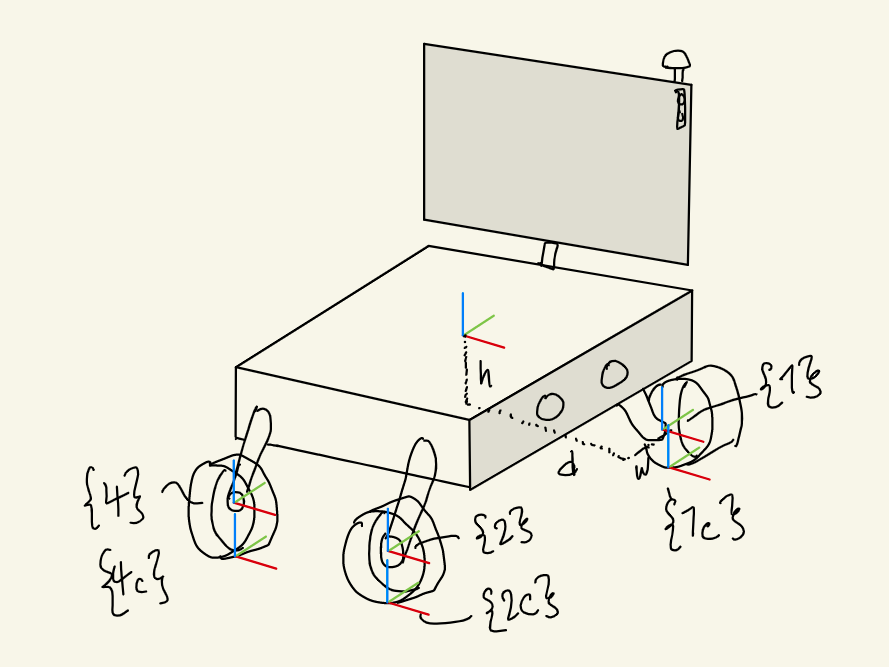
\includegraphics[width=0.5\textwidth]{images/frames.png}
    \caption{Frames of the wheel joints, and contact points.}
    \label{fig:frames}
\end{figure}
Using these transformations, we can obtain the actuation and navigation kinematics and use the transforms from wheels to the body of the rover and derive a wheel Jacobian $A$, which describes the change in wheel joint movements based off of body frame velocities. 
The wheel Jacobian is used to act on the rover state vector $q$:
\begin{equation}
q = \begin{bmatrix}   
\psi_x \\
\psi_y \\
\psi_z \\
x \\
y \\
z \\
\theta_1 \\
\theta_2 \\
\theta_3 \\
\theta_4
\end{bmatrix}
\end{equation}

The first six entries are the pose, and the last four are the joint values. 

The reason we need to know the wheel contact point frames is that we are going to enforce a "wheel contact velocity" $v_c$ constraint on the vehicle. 
This contact velocity constraint determines whether the wheel is slipping or not, and will be proportional to the rover speed, and the terrain parameters of the ground. 
The wheel contact constraint must satisfy the following equation involving the wheel Jacobian $A_i$. 
\begin{align}
    v_c &= \begin{bmatrix}
    v_x \\
    v_y \\
    v_z
    \end{bmatrix}\\
   A_i \dot{q} &= v_c
   \label{eq: wheel contact}
\end{align}
The wheel contact constraint models slip as an adjustment of the rover pose in the world frame, which is partially why we use a state vector that includes both the pose and wheel velocities on top of each other. 
For example if slip is 0 then all the $v_x, v_y$ entries in the constraint vector are 0, meaning no deviation occurs in these directions in the overall system. 
This is shown in figure \ref{fig:contact}.
\begin{figure}
    \centering
    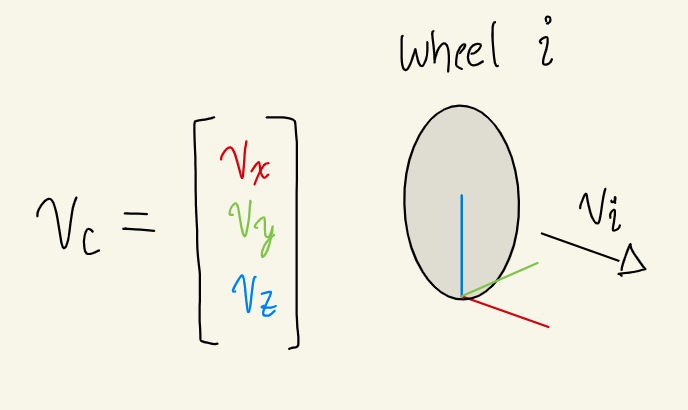
\includegraphics[width=0.5\textwidth]{images/wheel_contact.png}
    \caption{The contact frame of the wheel used to estimate slip.}
    \label{fig:contact}
\end{figure}

The Jacobian $A_i$ will be of size $3 \times 10$, due to the wheel contact constraint we enforce in equation \ref{eq: wheel contact}. 
For wheel $i$ the formulation of the wheel Jacobian $A_i$ is as follows:
\begin{align}
    \Theta_i &\in \mathbb{R}^{3 \times 4}\\
    \Theta_i[:, i] &= R^w_i[:, a(i)] \times (r^w_c - r^w_i)\\
    A_i &= \begin{bmatrix}
    [r^w_c - r^w_1]_{\times}^T R^w_1 & R^w_1 & \Theta_i 
    \end{bmatrix}
\end{align}
Where $\Theta_i$ is the joint Jacobian of wheel $i$, $a(i)$ is the axis of rotation of the joint $i$, $R^a_b$ is the rotation matrix from frame $b$ to frame $a$, and $r_b^a$ is the position vector in $x,y,z$ from frame $b$ to frame $a$; for example, $R_1^w$ is the transform of the body frame relative to the world frame. 
Note that $\Theta_i[:, i]$ means that we fill the $i^{th}$ column of $\Theta$ with the calculation $R^w_i[:, a(i)] \times (r^w_c - r^w_i)$.
We can form the full system Jacobian $A$ by stacking the four wheel Jacobians horizontally. 
Lastly we perform a transform on the Jacobian from world to contact coordinates, $A = (R^w_c)^T A $ in order to ensure that the Jacobian produces the relevant output from actuation or navigation kinematics in the rover frame. 

Now to actually compute the actuation or navigation kinematics, we use our constraint from earlier, and apply the pseudo-inverse of the Jacobian, like so: 
\begin{equation}
    \dot{q(unknown)} = A[:, unknown]^{\dagger} (v_c - A[:, known] \dot{q}(known))
\end{equation}
Here {\it unknown} and {\it known} describe the parts of the state vector $q$ that we are trying to solve for. We can then slice up the Jacobian in order to solve for these unknowns. 
For example, when solving either kinematic direction (actuation or navigation) we solve one of the following equations:
\begin{align}
    \dot{\theta} &= A_u^{\dagger} (v_c - A_k v^w_b) \label{eq: actuation}\\
    v^w_b &= A_u^{\dagger} (v_c - A_k \dot{\theta}) \label{eq: navigation}
\end{align}

where $\dot{\theta}$ is the joint rate, $v^w_b$ is the desired body velocities, $A_u, A_k$ are the sliced up Jacobians corresponding to the pose and joint values, and $v_c$ is the contact velocity constraint from equation \ref{eq: wheel contact}. 

\section{Implementation}
The approach detailed in the previous section and in \cite{Seegmiller-2014-7945} is meant to function as a general approach to solving 3D kinematics for wheeled mobile robots given and vehicle geometry with both fixed and free link joints. 
Seegmiller's formulation is essentially a 6 step process consisting of these steps: 
\begin{enumerate}
    \item Use the current joint positions to construct the list of transforms to each joint $i$ and each contact frame $c$
    \item Use the list of transforms to construct the current Jacobian matrix $A$
    \item Solve either for the actuation kinematics (joint velocities) or navigation kinematics (body velocity)
    \item Use the calculated joint or body velocity to inform state update of rover
    \item Assemble the state vector and propagate vehicle state through time
    \item Repeat from step 1
\end{enumerate}

However when we apply this to MoonRanger, there is key information that we know will stay constant throughout the mission, which invites an oppurtunity to simplify the original problem. 
This includes various dimensions of Moonranger, and the fact that Moonranger is a four wheeled skid steer vehicle. 
In addition, we made the simplifying assumption earlier that the wheel contact frame is fixed at the wheel radius directly beneath the wheel hub, and does not change throughout the mission. 
This assumption sacrifices accuracy in order to gain computational ease. 
It is also not necessary for the kinematic model to maintain a 3D state of the rover, because this is performed by the state estimator module. 
This means that we can potentially skip most of the steps of the previous list and only proceed with steps 3 and 4. 

The main benefit of simplifying this in this manner is that is drastically reduces the amount of online computation required to perform the four wheeled kinematics, nor do we need to concern ourselves with detailing this information in the Jacobian. 
Therefore we can simplify the problem like so:
\begin{enumerate}
    \item Determine the symbolic form of the Jacobian required to calculate kinematics
    \item Use this Jacobian to calculate the form of the pseudo-inverses, again simplifying online computation
    \item Solve either actuation or navigation kinematics and output result
\end{enumerate}

First, to find the symbolic form of the Jacobian. 
Because the algorithm produces a Jacobian in the contact frame coordinates as opposed to the world coordinates, the values are stable throughout the journey of the rover. 
Knowing this, we can produce the Jacobian like so:
\begin{equation}
    A_{moonranger} =
    \begin{bmatrix}
0 & - h - r& -w& 1& 0& 0& -r&  0&  0&  0\\
h + r& 0&  l& 0& 1& 0&  0&  0&  0&  0\\
w & -l& 0& 0& 0& 1&  0&  0&  0&  0\\
0& -h - r&  w& 1& 0& 0&  0& -r&  0&  0\\
h + r&0&  l& 0& 1& 0&  0&  0&  0&  0\\
-w&-l&0& 0& 0& 1&  0&  0&  0&  0\\
0& - h - r& -w& 1& 0& 0&  0&  0& -r&  0\\
h + r&0& -l& 0& 1& 0&  0&  0&  0&  0\\
w&l&0& 0& 0& 1&  0&  0&  0&  0\\
0& - h - r&  w& 1& 0& 0&  0&  0&  0& -r\\
h + r&0& -l& 0& 1& 0&  0&  0&  0&  0\\
-w&l&0& 0& 0& 1&  0&  0&  0&  0]\\
    \end{bmatrix}
\end{equation}
After the Jacobian is determined, we can cache the pseudo inverse of the velocity and joint rate Jacobians required for the computation in equations \ref{eq: actuation} and \ref{eq: navigation}. 
This means that the kinematics in either direction becomes as simple as a single matrix multiplication.

Notice that the Jacobian here doesn't include any sort of trigonometry even though it's construction uses several different rotation matrices. 
This is a direct result of Moonranger being skid-steered. If the joints were able to swivel, or the joint frames arranged at certain offsets from the body frame, this Jacobian would be more complicated, though similarly static. 
Results of using this Jacobian to calculate velocity kinematics and then updating the vehicle's state through time are shown in figure \ref{fig:static1}, which was generated in Matlab. 

\begin{figure}
    \centering
    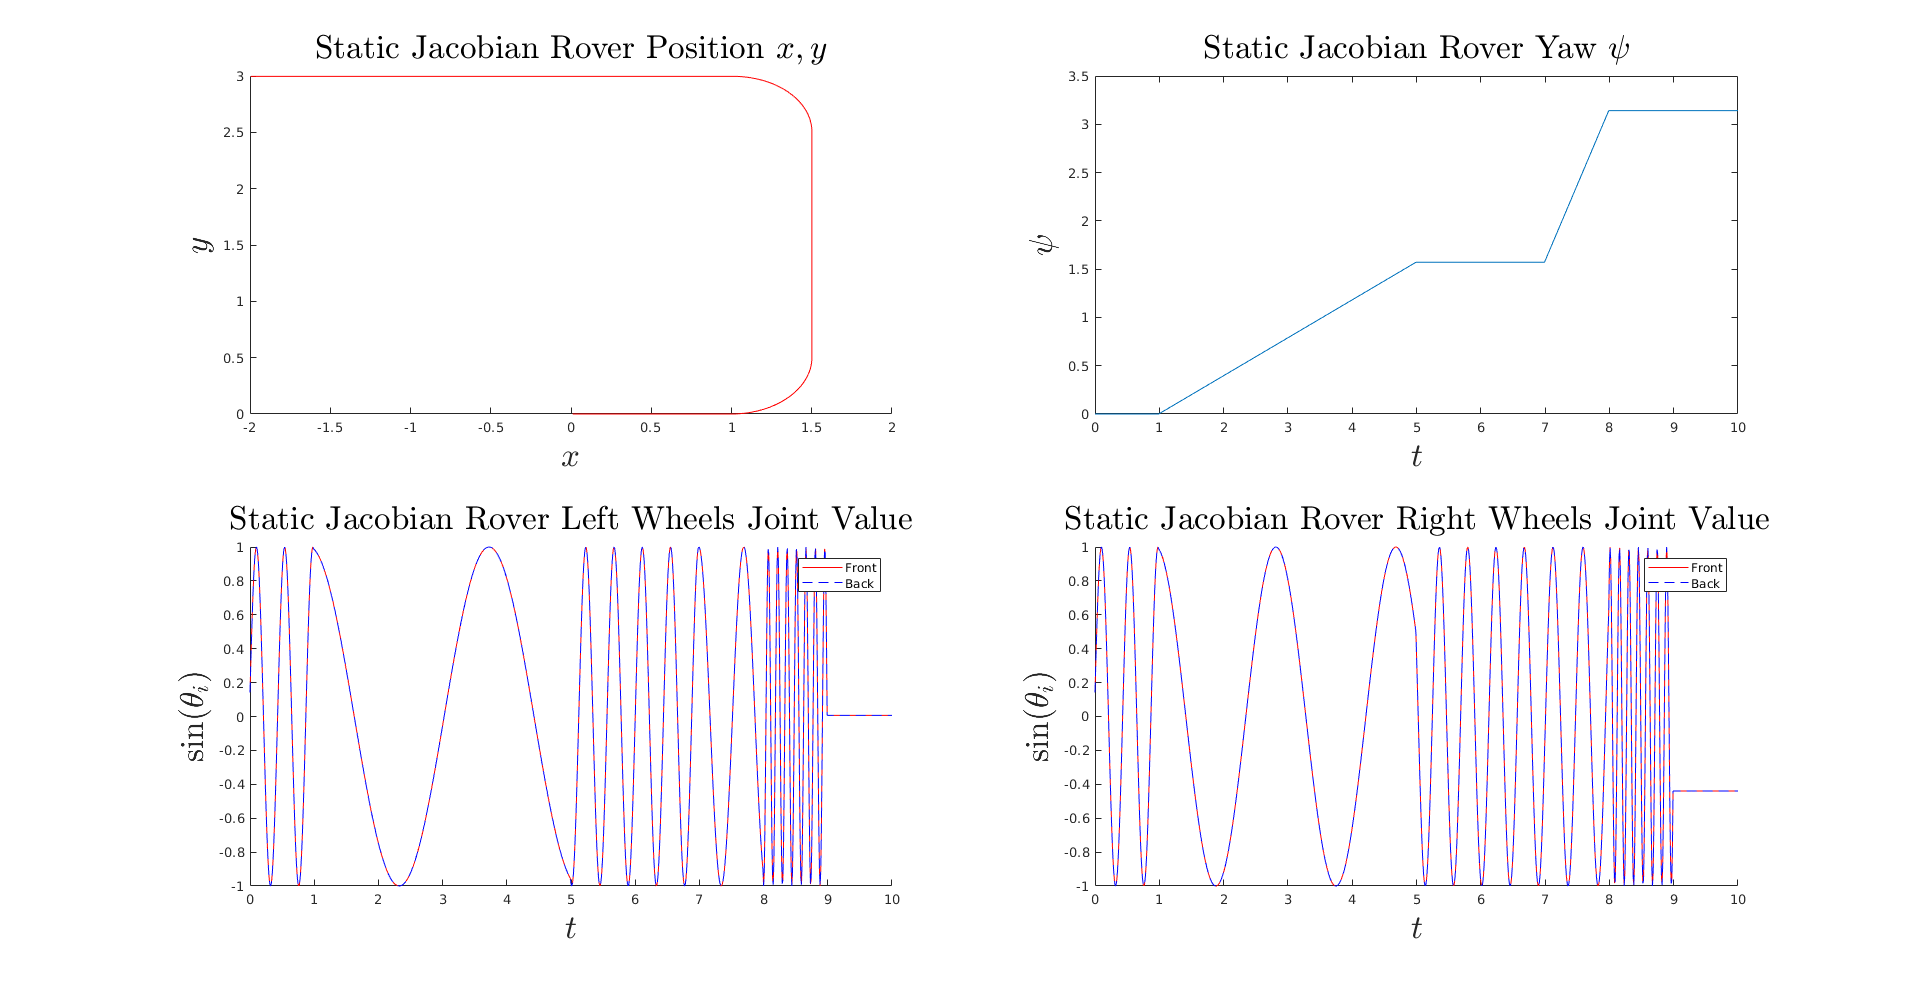
\includegraphics[width=\textwidth]{images/staticJacobianLeftTurn1.png}
    \caption{Results of the kinematic model being told to perform a couple drive arcs. Notice how the model is able to produce different speeds for individual wheels.}
    \label{fig:static1}
\end{figure}
Now that the Jacobian and its slices and pseudoinverse are known, the implementation can work as shown by the architecture in figure \ref{fig:code}.

\begin{figure}
    \centering
    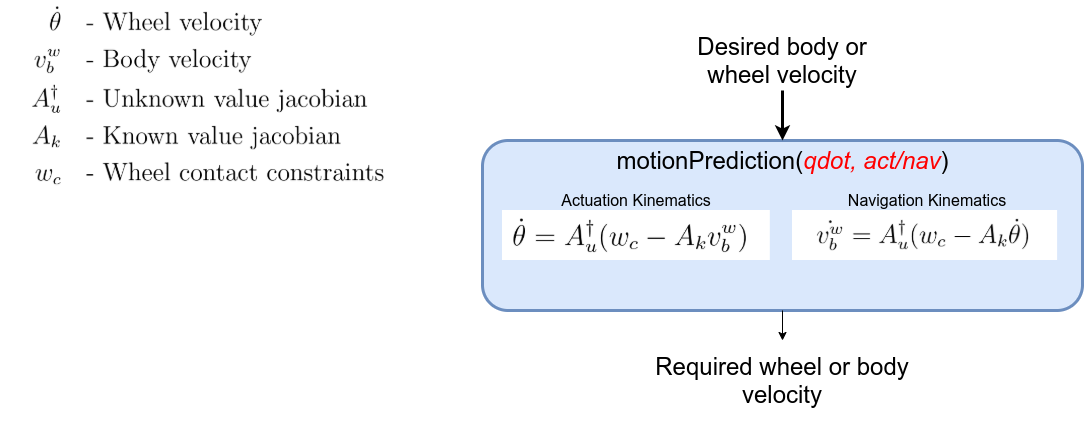
\includegraphics[width=\textwidth]{images/controller_architecture.png}
    \caption{The kinematics code flow architecture.}
    \label{fig:code}
\end{figure}
\break
\appendix
\section{Proof of Jacobian Simplification}

Recall from earlier that the formula for the Jacobian of wheel $i$ is 
\begin{align}
    \Theta_i &\in \mathbb{R}^{3 \times 4}\\
    \Theta_i[:, i] &= R^w_i[:, a(i)] \times (r^w_c - r^w_i)\\
    A_i &= \begin{bmatrix}
    [r^w_c - r^w_1]_{\times}^T R^w_1 & R^w_1 & \Theta_i 
    \end{bmatrix}
\end{align}
Which is then assembled into the Jacobian for all four wheels $A$, and multiplied by the rotation matrix $A = (R_c^w)^T A$ which rotates the entire Jacobian into the contact frame of the rover. 
If we then apply this rotation to each individual part of the wheel Jacobian:
\begin{align}
    R_w^c \left( [r^w_c - r^w_1]^T_{\times} R^w_1 \right) &= R^c_w (r_1^w - r^w_c) \times R^c_w R_1^w \\
    &= (R_w^c r_1^w - R_w^c r_c^w) \times R^c_1 \\
    &= (r^c_1 - r^c_c) \times R^c_1 \\
    &= r^c_1 \times R_1^c
\end{align}
We can see that this cross product is an expression of the contact to the base frame of wheel $i$. 
The middle matrix is simple: $R_w^c R^w_1 = R^c_1$, another matrix referencing contact frame from body frame. 
Lastly, the joint angle portion of the Jacobian:
\begin{align}
    R^c_w \Big(R_i^w[:, a(i)] \times (r_c^w - r^w_i)\Big) &= R_w^c R_i^w[:, a(i)] \times (R_w^c r_c^w - R_w^c r_i^w) \\
    &= R^c_i[:, a(i)] \times (r^c_c - r^c_i)
\end{align}
So we now have expressions for the wheel Jacobian in the contact frame. 
The key assumption enabling this simplification is that the contact frame does not change with respect to the rover and therefore, the Jacobian can be treated as static. 
Without this assumption, this simplification does not hold, and the Jacobian would need to be recalculated in accordance with the current contact frame and joint angle. 
It is possible to model the contact frame as moving with the terrain, but that would require interfacing with the mapper to generate terrain contact points on the mesh, which would require more functionality be added to the vehicle controller and ultimately further complicate the system. 

% Example of using bib like \cite{BRIEF}. 
\bibliographystyle{unsrt}
\bibliography{bib}
\end{document}
